% Section 1 - Containers
% Roberto Masocco <roberto.masocco@uniroma2.it>
% May 1, 2022

% ### Containers ###
\section{Containers}
\graphicspath{{figs/section1/}}

% --- Why Containers? ---
\begin{frame}{Why Containers?}
\begin{exampleblock}{Example: Packaging Applications}
  Suppose you are ready to distribute your new application:
  \begin{itemize}
    \item you need to be sure that it is compatible with all the \textbf{platforms} you chose to support;
    \item you need to figure out a way to deal with \textbf{dependencies};
    \item you want to publish some kind of self-contained, easily-identifiable \textbf{package}.
  \end{itemize}
\end{exampleblock}
\end{frame}
\begin{frame}{Why Containers?}
\begin{exampleblock}{Example: Isolating Applications}
  Suppose you are deploying applications on a server:
  \begin{itemize}
    \item you want to define \textbf{resource quotas} and \textbf{permissions} for each;
    \item you want to be sure that each module has what it needs to operate, but \textbf{nothing more};
    \item you want to \textbf{isolate} each module for security reasons, in case something goes wrong.
  \end{itemize}
\end{exampleblock}
\end{frame}
\begin{frame}{Why Containers?}
\begin{exampleblock}{Example: Replicating Environments}
  Suppose you are developing applications for a specific system (maybe with a different architecture):
  \begin{itemize}
    \item you want to have a \textbf{local copy} of such system without carrying one with you;
    \item you want to have all \textbf{libraries} and \textbf{dependencies} installed without tainting your own system;
    \item you would like to \textbf{deploy} the entire installation with just a few commands, without running any script but simply copying data.
  \end{itemize}
\end{exampleblock}
\end{frame}
\begin{frame}{Why Containers?}
\begin{columns}
  \column{.5\textwidth}
  A possible solution to many of the previous situations could be a set of \textbg{virtual machines}.\\
  However, virtual machines are \textbg{slow}, hypervisors take up \textbg{system resources} and guest kernels must always be \textbg{tweaked}.\\
  In each of the above scenarios something simpler would be enough, especially since \textbg{the OS is not involved}, only applications are.\\
  \begin{block}{}
    \centering
    This is what a \textbf{container} is.
  \end{block}

  \column{.5\textwidth}
  \begin{figure}
    \centering
    
\includegraphics[scale=.7]{freebsdjail.png}
    \label{fig:jail}
    \caption{FreeBSD jail logo}
  \end{figure}
\end{columns}
\end{frame}

% --- Containers in the Linux kernel ---
\begin{frame}{Containers in the Linux kernel}
\begin{columns}
  \column{.5\textwidth}
  Support for containers was added to the Linux kernel with a set of \textbg{features} starting from kernel 2.6 (2003), mainly:
  \begin{itemize}
    \item \textbg{control groups} (\texttt{cgroups}): defining different resource usage policies for groups of processes;
    \item \textbg{namespaces}: isolating processes and users in different "realms", both hardware (e.g. network stack) and software (e.g. PIDs);
    \item \textbg{capabilities}: granting some of the superuser's permissions to unprivileged threads.
  \end{itemize}

  \column{.5\textwidth}
  \begin{figure}
    \centering
    
\includegraphics[scale=.2]{tux.png}
    \label{fig:tux}
    \caption{Tux}
  \end{figure}
\end{columns}
\end{frame}
\begin{frame}{Containers in the Linux kernel}
\begin{figure}
  \centering
  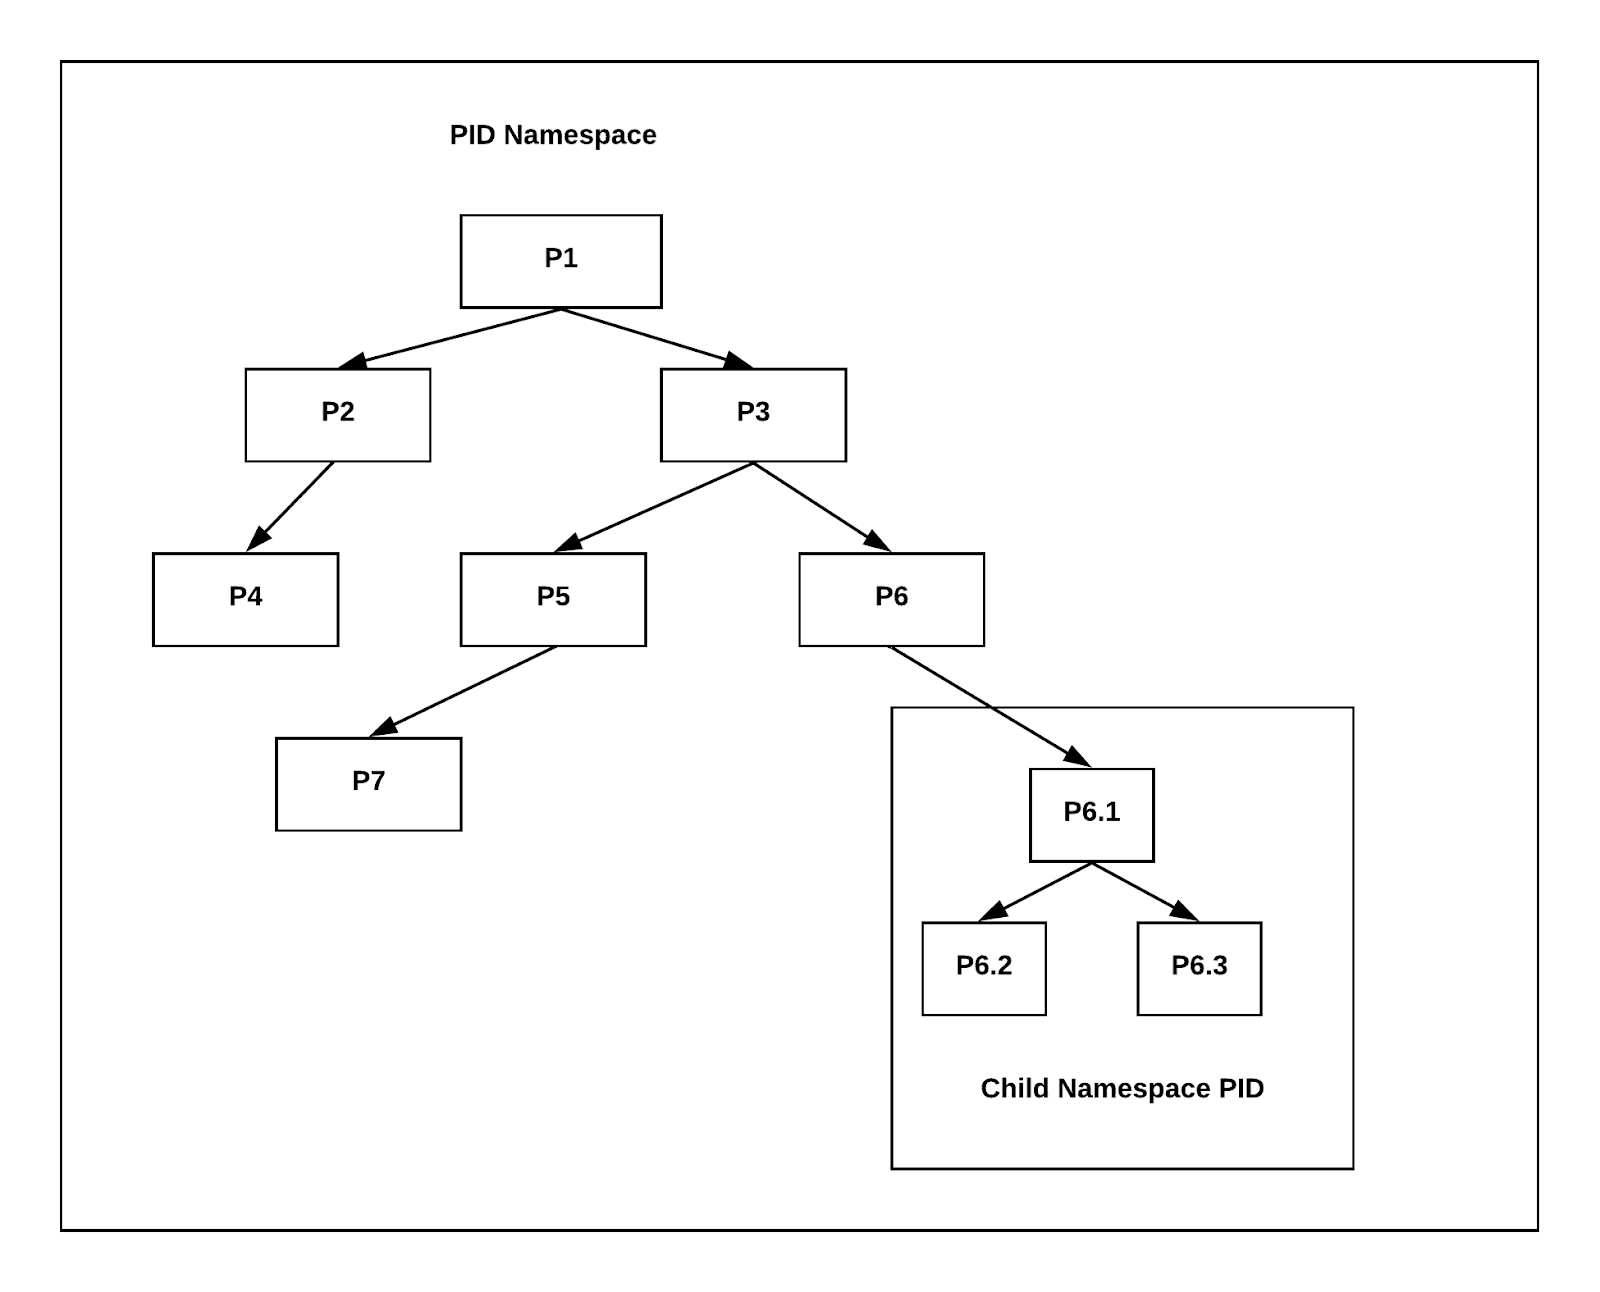
\includegraphics[scale=.15]{pidNamespace.png}
  \label{fig:pidnamespace}
  \caption{Nested PID namespaces}
\end{figure}
\end{frame}
